% Options for packages loaded elsewhere
\PassOptionsToPackage{unicode}{hyperref}
\PassOptionsToPackage{hyphens}{url}
\PassOptionsToPackage{dvipsnames,svgnames,x11names}{xcolor}
%
\documentclass[
  letterpaper,
  DIV=11,
  numbers=noendperiod]{scrartcl}

\usepackage{amsmath,amssymb}
\usepackage{iftex}
\ifPDFTeX
  \usepackage[T1]{fontenc}
  \usepackage[utf8]{inputenc}
  \usepackage{textcomp} % provide euro and other symbols
\else % if luatex or xetex
  \usepackage{unicode-math}
  \defaultfontfeatures{Scale=MatchLowercase}
  \defaultfontfeatures[\rmfamily]{Ligatures=TeX,Scale=1}
\fi
\usepackage{lmodern}
\ifPDFTeX\else  
    % xetex/luatex font selection
\fi
% Use upquote if available, for straight quotes in verbatim environments
\IfFileExists{upquote.sty}{\usepackage{upquote}}{}
\IfFileExists{microtype.sty}{% use microtype if available
  \usepackage[]{microtype}
  \UseMicrotypeSet[protrusion]{basicmath} % disable protrusion for tt fonts
}{}
\makeatletter
\@ifundefined{KOMAClassName}{% if non-KOMA class
  \IfFileExists{parskip.sty}{%
    \usepackage{parskip}
  }{% else
    \setlength{\parindent}{0pt}
    \setlength{\parskip}{6pt plus 2pt minus 1pt}}
}{% if KOMA class
  \KOMAoptions{parskip=half}}
\makeatother
\usepackage{xcolor}
\setlength{\emergencystretch}{3em} % prevent overfull lines
\setcounter{secnumdepth}{-\maxdimen} % remove section numbering
% Make \paragraph and \subparagraph free-standing
\makeatletter
\ifx\paragraph\undefined\else
  \let\oldparagraph\paragraph
  \renewcommand{\paragraph}{
    \@ifstar
      \xxxParagraphStar
      \xxxParagraphNoStar
  }
  \newcommand{\xxxParagraphStar}[1]{\oldparagraph*{#1}\mbox{}}
  \newcommand{\xxxParagraphNoStar}[1]{\oldparagraph{#1}\mbox{}}
\fi
\ifx\subparagraph\undefined\else
  \let\oldsubparagraph\subparagraph
  \renewcommand{\subparagraph}{
    \@ifstar
      \xxxSubParagraphStar
      \xxxSubParagraphNoStar
  }
  \newcommand{\xxxSubParagraphStar}[1]{\oldsubparagraph*{#1}\mbox{}}
  \newcommand{\xxxSubParagraphNoStar}[1]{\oldsubparagraph{#1}\mbox{}}
\fi
\makeatother

\usepackage{color}
\usepackage{fancyvrb}
\newcommand{\VerbBar}{|}
\newcommand{\VERB}{\Verb[commandchars=\\\{\}]}
\DefineVerbatimEnvironment{Highlighting}{Verbatim}{commandchars=\\\{\}}
% Add ',fontsize=\small' for more characters per line
\usepackage{framed}
\definecolor{shadecolor}{RGB}{241,243,245}
\newenvironment{Shaded}{\begin{snugshade}}{\end{snugshade}}
\newcommand{\AlertTok}[1]{\textcolor[rgb]{0.68,0.00,0.00}{#1}}
\newcommand{\AnnotationTok}[1]{\textcolor[rgb]{0.37,0.37,0.37}{#1}}
\newcommand{\AttributeTok}[1]{\textcolor[rgb]{0.40,0.45,0.13}{#1}}
\newcommand{\BaseNTok}[1]{\textcolor[rgb]{0.68,0.00,0.00}{#1}}
\newcommand{\BuiltInTok}[1]{\textcolor[rgb]{0.00,0.23,0.31}{#1}}
\newcommand{\CharTok}[1]{\textcolor[rgb]{0.13,0.47,0.30}{#1}}
\newcommand{\CommentTok}[1]{\textcolor[rgb]{0.37,0.37,0.37}{#1}}
\newcommand{\CommentVarTok}[1]{\textcolor[rgb]{0.37,0.37,0.37}{\textit{#1}}}
\newcommand{\ConstantTok}[1]{\textcolor[rgb]{0.56,0.35,0.01}{#1}}
\newcommand{\ControlFlowTok}[1]{\textcolor[rgb]{0.00,0.23,0.31}{\textbf{#1}}}
\newcommand{\DataTypeTok}[1]{\textcolor[rgb]{0.68,0.00,0.00}{#1}}
\newcommand{\DecValTok}[1]{\textcolor[rgb]{0.68,0.00,0.00}{#1}}
\newcommand{\DocumentationTok}[1]{\textcolor[rgb]{0.37,0.37,0.37}{\textit{#1}}}
\newcommand{\ErrorTok}[1]{\textcolor[rgb]{0.68,0.00,0.00}{#1}}
\newcommand{\ExtensionTok}[1]{\textcolor[rgb]{0.00,0.23,0.31}{#1}}
\newcommand{\FloatTok}[1]{\textcolor[rgb]{0.68,0.00,0.00}{#1}}
\newcommand{\FunctionTok}[1]{\textcolor[rgb]{0.28,0.35,0.67}{#1}}
\newcommand{\ImportTok}[1]{\textcolor[rgb]{0.00,0.46,0.62}{#1}}
\newcommand{\InformationTok}[1]{\textcolor[rgb]{0.37,0.37,0.37}{#1}}
\newcommand{\KeywordTok}[1]{\textcolor[rgb]{0.00,0.23,0.31}{\textbf{#1}}}
\newcommand{\NormalTok}[1]{\textcolor[rgb]{0.00,0.23,0.31}{#1}}
\newcommand{\OperatorTok}[1]{\textcolor[rgb]{0.37,0.37,0.37}{#1}}
\newcommand{\OtherTok}[1]{\textcolor[rgb]{0.00,0.23,0.31}{#1}}
\newcommand{\PreprocessorTok}[1]{\textcolor[rgb]{0.68,0.00,0.00}{#1}}
\newcommand{\RegionMarkerTok}[1]{\textcolor[rgb]{0.00,0.23,0.31}{#1}}
\newcommand{\SpecialCharTok}[1]{\textcolor[rgb]{0.37,0.37,0.37}{#1}}
\newcommand{\SpecialStringTok}[1]{\textcolor[rgb]{0.13,0.47,0.30}{#1}}
\newcommand{\StringTok}[1]{\textcolor[rgb]{0.13,0.47,0.30}{#1}}
\newcommand{\VariableTok}[1]{\textcolor[rgb]{0.07,0.07,0.07}{#1}}
\newcommand{\VerbatimStringTok}[1]{\textcolor[rgb]{0.13,0.47,0.30}{#1}}
\newcommand{\WarningTok}[1]{\textcolor[rgb]{0.37,0.37,0.37}{\textit{#1}}}

\providecommand{\tightlist}{%
  \setlength{\itemsep}{0pt}\setlength{\parskip}{0pt}}\usepackage{longtable,booktabs,array}
\usepackage{calc} % for calculating minipage widths
% Correct order of tables after \paragraph or \subparagraph
\usepackage{etoolbox}
\makeatletter
\patchcmd\longtable{\par}{\if@noskipsec\mbox{}\fi\par}{}{}
\makeatother
% Allow footnotes in longtable head/foot
\IfFileExists{footnotehyper.sty}{\usepackage{footnotehyper}}{\usepackage{footnote}}
\makesavenoteenv{longtable}
\usepackage{graphicx}
\makeatletter
\def\maxwidth{\ifdim\Gin@nat@width>\linewidth\linewidth\else\Gin@nat@width\fi}
\def\maxheight{\ifdim\Gin@nat@height>\textheight\textheight\else\Gin@nat@height\fi}
\makeatother
% Scale images if necessary, so that they will not overflow the page
% margins by default, and it is still possible to overwrite the defaults
% using explicit options in \includegraphics[width, height, ...]{}
\setkeys{Gin}{width=\maxwidth,height=\maxheight,keepaspectratio}
% Set default figure placement to htbp
\makeatletter
\def\fps@figure{htbp}
\makeatother

\usepackage{fvextra}
\DefineVerbatimEnvironment{Highlighting}{Verbatim}{breaklines,commandchars=\\\{\}}
\KOMAoption{captions}{tableheading}
\makeatletter
\@ifpackageloaded{caption}{}{\usepackage{caption}}
\AtBeginDocument{%
\ifdefined\contentsname
  \renewcommand*\contentsname{Table of contents}
\else
  \newcommand\contentsname{Table of contents}
\fi
\ifdefined\listfigurename
  \renewcommand*\listfigurename{List of Figures}
\else
  \newcommand\listfigurename{List of Figures}
\fi
\ifdefined\listtablename
  \renewcommand*\listtablename{List of Tables}
\else
  \newcommand\listtablename{List of Tables}
\fi
\ifdefined\figurename
  \renewcommand*\figurename{Figure}
\else
  \newcommand\figurename{Figure}
\fi
\ifdefined\tablename
  \renewcommand*\tablename{Table}
\else
  \newcommand\tablename{Table}
\fi
}
\@ifpackageloaded{float}{}{\usepackage{float}}
\floatstyle{ruled}
\@ifundefined{c@chapter}{\newfloat{codelisting}{h}{lop}}{\newfloat{codelisting}{h}{lop}[chapter]}
\floatname{codelisting}{Listing}
\newcommand*\listoflistings{\listof{codelisting}{List of Listings}}
\makeatother
\makeatletter
\makeatother
\makeatletter
\@ifpackageloaded{caption}{}{\usepackage{caption}}
\@ifpackageloaded{subcaption}{}{\usepackage{subcaption}}
\makeatother

\ifLuaTeX
  \usepackage{selnolig}  % disable illegal ligatures
\fi
\usepackage{bookmark}

\IfFileExists{xurl.sty}{\usepackage{xurl}}{} % add URL line breaks if available
\urlstyle{same} % disable monospaced font for URLs
\hypersetup{
  pdftitle={PS5 Andy Fan Will Sigal},
  colorlinks=true,
  linkcolor={blue},
  filecolor={Maroon},
  citecolor={Blue},
  urlcolor={Blue},
  pdfcreator={LaTeX via pandoc}}


\title{PS5 Andy Fan Will Sigal}
\author{}
\date{}

\begin{document}
\maketitle

\RecustomVerbatimEnvironment{verbatim}{Verbatim}{
  showspaces = false,
  showtabs = false,
  breaksymbolleft={},
  breaklines
}


\textbf{PS4:} Due Sat Nov 9 at 5:00PM Central. Worth 100 points.

\subsection{Style Points (10 pts)}\label{style-points-10-pts}

\subsection{Submission Steps (10 pts)}\label{submission-steps-10-pts}

\begin{enumerate}
\def\labelenumi{\arabic{enumi}.}
\tightlist
\item
  This problem set is a paired problem set.
\item
  Play paper, scissors, rock to determine who goes first. Call that
  person \emph{Partner 1}.

  \begin{itemize}
  \tightlist
  \item
    Partner 1 (name and cnet ID): Andy Fan, fanx
  \item
    Partner 2 (name and cnet ID): Will Sigal, Wsigal
  \end{itemize}
\item
  Partner 1 will accept the \texttt{ps5} and then share the link it
  creates with their partner. You can only share it with one partner so
  you will not be able to change it after your partner has accepted.
\item
  ``This submission is our work alone and complies with the 30538
  integrity policy.'' Add your initials to indicate your agreement:
\end{enumerate}

AF WS

\begin{enumerate}
\def\labelenumi{\arabic{enumi}.}
\setcounter{enumi}{4}
\tightlist
\item
  ``I have uploaded the names of anyone else other than my partner and I
  worked with on the problem set
  \textbf{\href{https://docs.google.com/forms/d/185usrCREQaUbvAXpWhChkjghdGgmAZXA3lPWpXLLsts/edit}{here}}''
  (1 point)
\item
  Late coins used this pset: (Andy:0); (Will:0) Late coins left after
  submission: (Andy: 3) ; (Will: 4)
\item
  Knit your \texttt{ps5.qmd} to an PDF file to make \texttt{ps5.pdf},

  \begin{itemize}
  \tightlist
  \item
    The PDF should not be more than 25 pages. Use \texttt{head()} and
    re-size figures when appropriate.
  \end{itemize}
\item
  (Partner 1): push \texttt{ps5.qmd} and \texttt{ps5.pdf} to your github
  repo.
\item
  (Partner 1): submit \texttt{ps5.pdf} via Gradescope. Add your partner
  on Gradescope.
\item
  (Partner 1): tag your submission in Gradescope
\end{enumerate}

\begin{Shaded}
\begin{Highlighting}[]
\CommentTok{\#\#\# SETUP }
\ImportTok{import}\NormalTok{ pandas }\ImportTok{as}\NormalTok{ pd}
\ImportTok{import}\NormalTok{ altair }\ImportTok{as}\NormalTok{ alt}
\ImportTok{import}\NormalTok{ time}
\ImportTok{import}\NormalTok{ os}
\ImportTok{import}\NormalTok{ warnings}
\ImportTok{import}\NormalTok{ geopandas }\ImportTok{as}\NormalTok{ gpd}
\ImportTok{import}\NormalTok{ numpy }\ImportTok{as}\NormalTok{ np}
\ImportTok{import}\NormalTok{ matplotlib.pyplot }\ImportTok{as}\NormalTok{ plt}
\NormalTok{warnings.filterwarnings(}\StringTok{\textquotesingle{}ignore\textquotesingle{}}\NormalTok{)}
\ImportTok{import}\NormalTok{ requests}
\ImportTok{from}\NormalTok{ bs4 }\ImportTok{import}\NormalTok{ BeautifulSoup}
\ImportTok{import}\NormalTok{ concurrent.futures}
\end{Highlighting}
\end{Shaded}

\subsection{(30 points) Step 1: Develop initial scraper and
crawler}\label{points-step-1-develop-initial-scraper-and-crawler}

\paragraph{1. (Partner 1) Scraping: Go to the first page of the HHS
OIG's ``Enforcement Actions''page and scrape and collect the following
into a dataset: • Title of the enforcement action • Date • Category
(e.g, ``Criminal and Civil Actions'') • Link associated with the
enforcement action Collect your output into a tidy dataframe and print
its
head.}\label{partner-1-scraping-go-to-the-first-page-of-the-hhs-oigs-enforcement-actionspage-and-scrape-and-collect-the-following-into-a-dataset-title-of-the-enforcement-action-date-category-e.g-criminal-and-civil-actions-link-associated-with-the-enforcement-action-collect-your-output-into-a-tidy-dataframe-and-print-its-head.}

\begin{Shaded}
\begin{Highlighting}[]
\CommentTok{\#\#\# making soup}
\NormalTok{url1 }\OperatorTok{=} \StringTok{\textquotesingle{}https://oig.hhs.gov/fraud/enforcement\textquotesingle{}}
\NormalTok{response1 }\OperatorTok{=}\NormalTok{ requests.get(url1)}
\NormalTok{soup1 }\OperatorTok{=}\NormalTok{ BeautifulSoup(response1.content, }\StringTok{\textquotesingle{}lxml\textquotesingle{}}\NormalTok{)}
\end{Highlighting}
\end{Shaded}

\begin{Shaded}
\begin{Highlighting}[]
\CommentTok{\#\#\# find title of enforcements}
\NormalTok{li\_blocks }\OperatorTok{=}\NormalTok{ soup1.find\_all(}\StringTok{\textquotesingle{}h2\textquotesingle{}}\NormalTok{) }\CommentTok{\# h2 classes with nested \textquotesingle{}a\textquotesingle{} titles. li\_blocks[2:21] are the 20 datapoints}
\NormalTok{li\_titles }\OperatorTok{=}\NormalTok{ []}
\ControlFlowTok{for}\NormalTok{ h2 }\KeywordTok{in}\NormalTok{ li\_blocks:}
    \ControlFlowTok{for}\NormalTok{ a\_tag }\KeywordTok{in}\NormalTok{ h2.find\_all(}\StringTok{\textquotesingle{}a\textquotesingle{}}\NormalTok{):}
\NormalTok{        li\_titles.append(a\_tag)}
\NormalTok{li\_titles[}\DecValTok{0}\NormalTok{:}\DecValTok{5}\NormalTok{]}
\NormalTok{df\_title }\OperatorTok{=}\NormalTok{ pd.DataFrame(li\_titles) }\CommentTok{\# dataframe with titles}
\NormalTok{df\_title.columns }\OperatorTok{=}\NormalTok{ [}\StringTok{\textquotesingle{}title\textquotesingle{}}\NormalTok{]}
\end{Highlighting}
\end{Shaded}

Title: each title is a `a' class, under h2 class. `h2 class' under
`header class' under `div class' under `li class'

\begin{Shaded}
\begin{Highlighting}[]
\CommentTok{\#\#\# find date}
\NormalTok{span\_blocks }\OperatorTok{=}\NormalTok{ soup1.find\_all(}\StringTok{\textquotesingle{}span\textquotesingle{}}\NormalTok{, attrs}\OperatorTok{=}\NormalTok{\{}\StringTok{\textquotesingle{}class\textquotesingle{}}\NormalTok{: }\StringTok{\textquotesingle{}text{-}base{-}dark padding{-}right{-}105\textquotesingle{}}\NormalTok{\})}
\NormalTok{span\_blocks[}\DecValTok{0}\NormalTok{:}\DecValTok{5}\NormalTok{]}
\NormalTok{df\_date }\OperatorTok{=}\NormalTok{ pd.DataFrame(span\_blocks) }
\NormalTok{df\_date.columns }\OperatorTok{=}\NormalTok{ [}\StringTok{\textquotesingle{}date\textquotesingle{}}\NormalTok{]}
\CommentTok{\#asked chat gpt \textquotesingle{}how to i search for \textquotesingle{}span\textquotesingle{} class with attribute xxx\textquotesingle{}}
\end{Highlighting}
\end{Shaded}

Date: is under `span' class

\begin{Shaded}
\begin{Highlighting}[]
\CommentTok{\#\#\# find category}
\NormalTok{li\_blocks\_dt }\OperatorTok{=}\NormalTok{ soup1.find\_all(}\StringTok{\textquotesingle{}li\textquotesingle{}}\NormalTok{, attrs}\OperatorTok{=}\NormalTok{\{}\StringTok{\textquotesingle{}class\textquotesingle{}}\NormalTok{: }\StringTok{\textquotesingle{}display{-}inline{-}block usa{-}tag text{-}no{-}lowercase text{-}base{-}darkest bg{-}base{-}lightest margin{-}right{-}1\textquotesingle{}}\NormalTok{\})}
\NormalTok{li\_blocks[}\DecValTok{0}\NormalTok{:}\DecValTok{5}\NormalTok{]}
\NormalTok{df\_category }\OperatorTok{=}\NormalTok{ pd.DataFrame(li\_blocks\_dt)}
\NormalTok{df\_category.columns }\OperatorTok{=}\NormalTok{ [}\StringTok{\textquotesingle{}category\textquotesingle{}}\NormalTok{]}
\end{Highlighting}
\end{Shaded}

Category: each category is a li class (search by attribute).'l1 class'
under `ul class' under `div class' under `header class'

\begin{Shaded}
\begin{Highlighting}[]
\CommentTok{\#\#\# find link}
\CommentTok{\#use the list of titles from p1 and extract href}
\NormalTok{link\_blocks }\OperatorTok{=}\NormalTok{ [link.get(}\StringTok{\textquotesingle{}href\textquotesingle{}}\NormalTok{) }\ControlFlowTok{for}\NormalTok{ link }\KeywordTok{in}\NormalTok{ li\_titles]}
\NormalTok{df\_link }\OperatorTok{=}\NormalTok{ pd.DataFrame(link\_blocks)}
\NormalTok{df\_link.columns }\OperatorTok{=}\NormalTok{ [}\StringTok{\textquotesingle{}link\textquotesingle{}}\NormalTok{]}
\NormalTok{df\_link[}\StringTok{\textquotesingle{}link\textquotesingle{}}\NormalTok{] }\OperatorTok{=} \StringTok{"https://oig.hhs.gov"} \OperatorTok{+}\NormalTok{ df\_link[}\StringTok{\textquotesingle{}link\textquotesingle{}}\NormalTok{] }\CommentTok{\#add front part of link to make it clickable}
\end{Highlighting}
\end{Shaded}

Link: link=href class, under h2 class. `h2 class' under `header class'
under `div class' under `li class'

\begin{Shaded}
\begin{Highlighting}[]
\CommentTok{\#\#\# combine dataframes}
\NormalTok{df\_Q1 }\OperatorTok{=}\NormalTok{ pd.concat([df\_title, df\_date, df\_category, df\_link], axis}\OperatorTok{=}\DecValTok{1}\NormalTok{)}
\BuiltInTok{print}\NormalTok{(df\_Q1.head())}
\end{Highlighting}
\end{Shaded}

\begin{verbatim}
                                               title              date  \
0  Pharmacist and Brother Convicted of $15M Medic...  November 8, 2024   
1  Boise Nurse Practitioner Sentenced To 48 Month...  November 7, 2024   
2  Former Traveling Nurse Pleads Guilty To Tamper...  November 7, 2024   
3  Former Arlington Resident Sentenced To Prison ...  November 7, 2024   
4  Paroled Felon Sentenced To Six Years For Fraud...  November 7, 2024   

                     category  \
0  Criminal and Civil Actions   
1  Criminal and Civil Actions   
2  Criminal and Civil Actions   
3  Criminal and Civil Actions   
4  Criminal and Civil Actions   

                                                link  
0  https://oig.hhs.gov/fraud/enforcement/pharmaci...  
1  https://oig.hhs.gov/fraud/enforcement/boise-nu...  
2  https://oig.hhs.gov/fraud/enforcement/former-t...  
3  https://oig.hhs.gov/fraud/enforcement/former-a...  
4  https://oig.hhs.gov/fraud/enforcement/paroled-...  
\end{verbatim}

\paragraph{2. (Partner 1) Crawling: Then for each enforcement action,
click the link and collect the name of the agency involved (e.g., for
this link, it would be U.S. Attorney's Office, Eastern District of
Washington).}\label{partner-1-crawling-then-for-each-enforcement-action-click-the-link-and-collect-the-name-of-the-agency-involved-e.g.-for-this-link-it-would-be-u.s.-attorneys-office-eastern-district-of-washington.}

\begin{Shaded}
\begin{Highlighting}[]
\CommentTok{\#\#\# webcrawl}
\NormalTok{urls\_1\_2 }\OperatorTok{=}\NormalTok{ df\_Q1[}\StringTok{\textquotesingle{}link\textquotesingle{}}\NormalTok{]}

\CommentTok{\#\#\# find agency by finding \textquotesingle{}li\textquotesingle{} tags nested in \textquotesingle{}article\textquotesingle{} tags}
\NormalTok{article\_tags }\OperatorTok{=}\NormalTok{ []}
\ControlFlowTok{for}\NormalTok{ url }\KeywordTok{in}\NormalTok{ urls\_1\_2:}
\NormalTok{    response }\OperatorTok{=}\NormalTok{ requests.get(url)}
    \ControlFlowTok{if}\NormalTok{ response.status\_code }\OperatorTok{==} \DecValTok{200}\NormalTok{:  }\CommentTok{\# Check if the request was successful}
\NormalTok{        soup }\OperatorTok{=}\NormalTok{ BeautifulSoup(response.text, }\StringTok{\textquotesingle{}html.parser\textquotesingle{}}\NormalTok{)}
        
        \CommentTok{\# Find all \textless{}articel\textgreater{} tags}
        \CommentTok{\#article\_tags = soup2.find\_all(\textquotesingle{}article\textquotesingle{})}
        
        \CommentTok{\# Find all \textless{}li\textgreater{} tags within \textless{}article\textgreater{} tags}
\NormalTok{        articles }\OperatorTok{=}\NormalTok{ soup.find\_all(}\StringTok{\textquotesingle{}article\textquotesingle{}}\NormalTok{)}
        \ControlFlowTok{for}\NormalTok{ article }\KeywordTok{in}\NormalTok{ articles:}
\NormalTok{            li\_tags }\OperatorTok{=}\NormalTok{ article.find\_all(}\StringTok{\textquotesingle{}li\textquotesingle{}}\NormalTok{)}
            \ControlFlowTok{for}\NormalTok{ li }\KeywordTok{in}\NormalTok{ li\_tags:}
\NormalTok{                article\_tags.append(li.get\_text(strip}\OperatorTok{=}\VariableTok{True}\NormalTok{))  }\CommentTok{\# Append the text of each \textless{}li\textgreater{} tag}
    \ControlFlowTok{else}\NormalTok{:}
        \BuiltInTok{print}\NormalTok{(}\SpecialStringTok{f"Failed to retrieve }\SpecialCharTok{\{}\NormalTok{link}\SpecialCharTok{\}}\SpecialStringTok{"}\NormalTok{)}

\CommentTok{\#\#\# make dataframe and remove non{-}relevant items from list}
\NormalTok{df\_agency }\OperatorTok{=}\NormalTok{ pd.DataFrame(article\_tags)}
\NormalTok{df\_agency.columns }\OperatorTok{=}\NormalTok{ [}\StringTok{\textquotesingle{}agency\textquotesingle{}}\NormalTok{]}
\NormalTok{df\_agency }\OperatorTok{=}\NormalTok{ df\_agency[df\_agency[}\StringTok{\textquotesingle{}agency\textquotesingle{}}\NormalTok{].}\BuiltInTok{str}\NormalTok{.contains(}\StringTok{\textquotesingle{}Agency\textquotesingle{}}\NormalTok{, case}\OperatorTok{=}\VariableTok{False}\NormalTok{, na}\OperatorTok{=}\VariableTok{False}\NormalTok{)]}

\BuiltInTok{print}\NormalTok{(df\_agency.head())}
\CommentTok{\#asked chat gpt \textquotesingle{}how to go to every link in a list and extracts all \textquotesingle{}li\textquotesingle{} tags that are nested in \textquotesingle{}article\textquotesingle{} tag and create them into a new list\textquotesingle{}}
\end{Highlighting}
\end{Shaded}

\begin{verbatim}
                                               agency
1                   Agency:U.S. Department of Justice
5   Agency:November 7, 2024; U.S. Attorney's Offic...
9   Agency:U.S. Attorney's Office, District of Mas...
13  Agency:U.S. Attorney's Office, Eastern Distric...
17  Agency:U.S. Attorney's Office, Middle District...
\end{verbatim}

Name of agency is `li' class, nested in `ul' nested in `div' nested in
`article'

*Some links do not have the corresponding agency listed, and a couple
(such as ``U.S. Attorney's Office, District of Idaho'' are not formatted
correctly)

\subsection{(30 points) Step 2: Making the scraper
dynamic}\label{points-step-2-making-the-scraper-dynamic}

\paragraph{1. Turning the scraper into a function: You will write a
function that takes as input a month and a year, and then pulls and
formats the enforcement actions like in Step 1 starting from that
month+year to
today.}\label{turning-the-scraper-into-a-function-you-will-write-a-function-that-takes-as-input-a-month-and-a-year-and-then-pulls-and-formats-the-enforcement-actions-like-in-step-1-starting-from-that-monthyear-to-today.}

\paragraph{a (Partner 2) Before writing out your function, write down
pseudo-code of the steps that your function will go through. If you use
a loop, discuss what kind of loop you will use and how you will define
it.}\label{a-partner-2-before-writing-out-your-function-write-down-pseudo-code-of-the-steps-that-your-function-will-go-through.-if-you-use-a-loop-discuss-what-kind-of-loop-you-will-use-and-how-you-will-define-it.}

\begin{Shaded}
\begin{Highlighting}[]
\CommentTok{\#1) Check if the year if the year is 2013 or later if not, terminte function}
\CommentTok{\#2) Create dictionary for params and use a while loop for pagnation setting for it to break when there\textquotesingle{}s no next.}
\CommentTok{\#3) Send Get request to get pages, dates, categories and links}
\CommentTok{\#4) append new info to our dictionary}
\CommentTok{\#5) wait one sec before going to the next page}
\end{Highlighting}
\end{Shaded}

\paragraph{b (Partner 2) Now code up your dynamic scraper and run it to
start collecting the enforcement actions since January 2023. How many
enforcement actions do you get in your final dataframe? What is the date
and details of the earliest enforcement action it
scraped?}\label{b-partner-2-now-code-up-your-dynamic-scraper-and-run-it-to-start-collecting-the-enforcement-actions-since-january-2023.-how-many-enforcement-actions-do-you-get-in-your-final-dataframe-what-is-the-date-and-details-of-the-earliest-enforcement-action-it-scraped}

\begin{Shaded}
\begin{Highlighting}[]
\ImportTok{import}\NormalTok{ time}
\ImportTok{from}\NormalTok{ datetime }\ImportTok{import}\NormalTok{ datetime}

\KeywordTok{def}\NormalTok{ enforcement\_scrapper(start\_month, start\_year):}
    \ControlFlowTok{if}\NormalTok{ start\_year }\OperatorTok{\textless{}} \DecValTok{2013}\NormalTok{:}
        \BuiltInTok{print}\NormalTok{(}\StringTok{"Please input a year \textgreater{}= 2013, as enforcement actions before 2013 are unavailable."}\NormalTok{)}
        \ControlFlowTok{return}

\NormalTok{    base\_url }\OperatorTok{=} \StringTok{\textquotesingle{}https://oig.hhs.gov/fraud/enforcement\textquotesingle{}}
\NormalTok{    current\_page }\OperatorTok{=} \DecValTok{1}
\NormalTok{    results }\OperatorTok{=}\NormalTok{ []}

    \ControlFlowTok{while} \VariableTok{True}\NormalTok{:}
\NormalTok{        url }\OperatorTok{=} \SpecialStringTok{f"}\SpecialCharTok{\{}\NormalTok{base\_url}\SpecialCharTok{\}}\SpecialStringTok{/?page=}\SpecialCharTok{\{}\NormalTok{current\_page}\SpecialCharTok{\}}\SpecialStringTok{"}
\NormalTok{        response }\OperatorTok{=}\NormalTok{ requests.get(url)}
\NormalTok{        soup }\OperatorTok{=}\NormalTok{ BeautifulSoup(response.content, }\StringTok{\textquotesingle{}lxml\textquotesingle{}}\NormalTok{)}
\CommentTok{\#titles links}
\NormalTok{        titles }\OperatorTok{=}\NormalTok{ []}
\NormalTok{        links }\OperatorTok{=}\NormalTok{ []}
        \ControlFlowTok{for}\NormalTok{ h2 }\KeywordTok{in}\NormalTok{ soup.find\_all(}\StringTok{\textquotesingle{}h2\textquotesingle{}}\NormalTok{):}
\NormalTok{            a\_tag }\OperatorTok{=}\NormalTok{ h2.find(}\StringTok{\textquotesingle{}a\textquotesingle{}}\NormalTok{)}
            \ControlFlowTok{if}\NormalTok{ a\_tag:}
\NormalTok{                titles.append(a\_tag.get\_text(strip}\OperatorTok{=}\VariableTok{True}\NormalTok{))}
\NormalTok{                links.append(}\StringTok{"https://oig.hhs.gov"} \OperatorTok{+}\NormalTok{ a\_tag[}\StringTok{\textquotesingle{}href\textquotesingle{}}\NormalTok{])}

        \CommentTok{\#get dates}
\NormalTok{        dates }\OperatorTok{=}\NormalTok{ [span.get\_text(strip}\OperatorTok{=}\VariableTok{True}\NormalTok{) }\ControlFlowTok{for}\NormalTok{ span }\KeywordTok{in}\NormalTok{ soup.find\_all(}\StringTok{\textquotesingle{}span\textquotesingle{}}\NormalTok{, class\_}\OperatorTok{=}\StringTok{\textquotesingle{}text{-}base{-}dark padding{-}right{-}105\textquotesingle{}}\NormalTok{)]}

        \CommentTok{\#get categories}
\NormalTok{        categories }\OperatorTok{=}\NormalTok{ [}
\NormalTok{            li.get\_text(strip}\OperatorTok{=}\VariableTok{True}\NormalTok{) }\ControlFlowTok{for}\NormalTok{ li }\KeywordTok{in}\NormalTok{ soup.find\_all(}\StringTok{\textquotesingle{}li\textquotesingle{}}\NormalTok{, class\_}\OperatorTok{=}\StringTok{\textquotesingle{}display{-}inline{-}block usa{-}tag text{-}no{-}lowercase text{-}base{-}darkest bg{-}base{-}lightest margin{-}right{-}1\textquotesingle{}}\NormalTok{)}
\NormalTok{        ]}

        \ControlFlowTok{for}\NormalTok{ title, date, category, link }\KeywordTok{in} \BuiltInTok{zip}\NormalTok{(titles, dates, categories, links):}
\NormalTok{            results.append(\{}\StringTok{\textquotesingle{}Title\textquotesingle{}}\NormalTok{: title, }\StringTok{\textquotesingle{}Date\textquotesingle{}}\NormalTok{: date, }\StringTok{\textquotesingle{}Category\textquotesingle{}}\NormalTok{: category, }\StringTok{\textquotesingle{}Link\textquotesingle{}}\NormalTok{: link\})}

        \CommentTok{\#check if page has dates earlier than when we\textquotesingle{}re looking}
\NormalTok{        date\_check }\OperatorTok{=}\NormalTok{ pd.to\_datetime(dates, errors}\OperatorTok{=}\StringTok{\textquotesingle{}coerce\textquotesingle{}}\NormalTok{)}
        \ControlFlowTok{if}\NormalTok{ date\_check.}\BuiltInTok{min}\NormalTok{() }\OperatorTok{\textless{}}\NormalTok{ pd.Timestamp(datetime(start\_year, start\_month, }\DecValTok{1}\NormalTok{)):}
            \ControlFlowTok{break}
        
\NormalTok{        current\_page }\OperatorTok{+=} \DecValTok{1}


        
\NormalTok{        time.sleep(}\DecValTok{1}\NormalTok{)}

    
\NormalTok{    scrapper }\OperatorTok{=}\NormalTok{ pd.DataFrame(results)}
\NormalTok{    scrapper[}\StringTok{\textquotesingle{}Date\textquotesingle{}}\NormalTok{] }\OperatorTok{=}\NormalTok{ pd.to\_datetime(scrapper[}\StringTok{\textquotesingle{}Date\textquotesingle{}}\NormalTok{])}
\NormalTok{    start\_date }\OperatorTok{=}\NormalTok{ datetime(start\_year, start\_month, }\DecValTok{1}\NormalTok{)}
\NormalTok{    scrapper }\OperatorTok{=}\NormalTok{ scrapper[scrapper[}\StringTok{\textquotesingle{}Date\textquotesingle{}}\NormalTok{] }\OperatorTok{\textgreater{}=}\NormalTok{ start\_date]}
    \ControlFlowTok{return}\NormalTok{ scrapper}
\end{Highlighting}
\end{Shaded}

\begin{Shaded}
\begin{Highlighting}[]
\NormalTok{twenty\_three }\OperatorTok{=}\NormalTok{ enforcement\_scrapper(}\DecValTok{1}\NormalTok{, }\DecValTok{2023}\NormalTok{)  }

\BuiltInTok{print}\NormalTok{(twenty\_three.shape[}\DecValTok{0}\NormalTok{])}
\end{Highlighting}
\end{Shaded}

\begin{verbatim}
1534
\end{verbatim}

\begin{Shaded}
\begin{Highlighting}[]
\NormalTok{earliest\_date }\OperatorTok{=}\NormalTok{ twenty\_three[}\StringTok{\textquotesingle{}Date\textquotesingle{}}\NormalTok{].}\BuiltInTok{min}\NormalTok{()}
\BuiltInTok{print}\NormalTok{(}\SpecialStringTok{f"Earliest Date: }\SpecialCharTok{\{}\NormalTok{earliest\_date}\SpecialCharTok{.}\NormalTok{date()}\SpecialCharTok{\}}\SpecialStringTok{"}\NormalTok{)}

\NormalTok{num\_enforcements }\OperatorTok{=} \BuiltInTok{len}\NormalTok{(twenty\_three)}
\BuiltInTok{print}\NormalTok{(}\SpecialStringTok{f"Number of Enforcement Actions: }\SpecialCharTok{\{}\NormalTok{num\_enforcements}\SpecialCharTok{\}}\SpecialStringTok{"}\NormalTok{)}
\end{Highlighting}
\end{Shaded}

\begin{verbatim}
Earliest Date: 2023-01-03
Number of Enforcement Actions: 1534
\end{verbatim}

\paragraph{c (Partner 1) Now, let's go a little further back. Test your
partner's code by collecting the actions since January 2021. Note that
this can take a while. How many enforcement actions do you get in your
final dataframe? What is the date and details of the earliest
enforcement action it scraped? Use the dataframe from this process for
every question after
this}\label{c-partner-1-now-lets-go-a-little-further-back.-test-your-partners-code-by-collecting-the-actions-since-january-2021.-note-that-this-can-take-a-while.-how-many-enforcement-actions-do-you-get-in-your-final-dataframe-what-is-the-date-and-details-of-the-earliest-enforcement-action-it-scraped-use-the-dataframe-from-this-process-for-every-question-after-this}

\begin{Shaded}
\begin{Highlighting}[]
\NormalTok{twenty\_one }\OperatorTok{=}\NormalTok{ enforcement\_scrapper(}\DecValTok{1}\NormalTok{, }\DecValTok{2021}\NormalTok{)}
\NormalTok{num\_enforcements }\OperatorTok{=} \BuiltInTok{len}\NormalTok{(twenty\_one)}
\end{Highlighting}
\end{Shaded}

\begin{Shaded}
\begin{Highlighting}[]
\CommentTok{\#my code was taking me far far too long and so I used chat gpt to find how I can increase the speed of my crawler}
\ImportTok{import}\NormalTok{ concurrent.futures}
\KeywordTok{def}\NormalTok{ scrape\_link(link):}
    \ControlFlowTok{try}\NormalTok{:}
\NormalTok{        response }\OperatorTok{=}\NormalTok{ requests.get(link)}
\NormalTok{        detail\_soup }\OperatorTok{=}\NormalTok{ BeautifulSoup(response.content, }\StringTok{\textquotesingle{}lxml\textquotesingle{}}\NormalTok{)}
\NormalTok{        agency\_label }\OperatorTok{=}\NormalTok{ detail\_soup.find(}\StringTok{\textquotesingle{}span\textquotesingle{}}\NormalTok{, class\_}\OperatorTok{=}\StringTok{\textquotesingle{}padding{-}right{-}2 text{-}base\textquotesingle{}}\NormalTok{, text}\OperatorTok{=}\StringTok{\textquotesingle{}Agency:\textquotesingle{}}\NormalTok{)}
        \ControlFlowTok{if}\NormalTok{ agency\_label:}
            \CommentTok{\# Get the actual text that follows the Agency: label}
\NormalTok{            agency\_text }\OperatorTok{=}\NormalTok{ agency\_label.next\_sibling}
            \ControlFlowTok{if}\NormalTok{ agency\_text:}
                \ControlFlowTok{return}\NormalTok{ agency\_text.strip()}
        \ControlFlowTok{return} \VariableTok{None}
    \ControlFlowTok{except} \PreprocessorTok{Exception} \ImportTok{as}\NormalTok{ e:}
        \BuiltInTok{print}\NormalTok{(}\SpecialStringTok{f"Error scraping }\SpecialCharTok{\{}\NormalTok{link}\SpecialCharTok{\}}\SpecialStringTok{: }\SpecialCharTok{\{}\NormalTok{e}\SpecialCharTok{\}}\SpecialStringTok{"}\NormalTok{)}
        \ControlFlowTok{return} \VariableTok{None}

\KeywordTok{def}\NormalTok{ main():}
    \ControlFlowTok{with}\NormalTok{ concurrent.futures.ThreadPoolExecutor(max\_workers}\OperatorTok{=}\DecValTok{10}\NormalTok{) }\ImportTok{as}\NormalTok{ executor:}
\NormalTok{        futures }\OperatorTok{=}\NormalTok{ \{executor.submit(scrape\_link, link): link }\ControlFlowTok{for}\NormalTok{ link }\KeywordTok{in}\NormalTok{ twenty\_one[}\StringTok{\textquotesingle{}Link\textquotesingle{}}\NormalTok{]\}}
\NormalTok{        agencies }\OperatorTok{=}\NormalTok{ [future.result() }\ControlFlowTok{for}\NormalTok{ future }\KeywordTok{in}\NormalTok{ futures]}

\NormalTok{    twenty\_one[}\StringTok{\textquotesingle{}Agency\textquotesingle{}}\NormalTok{] }\OperatorTok{=}\NormalTok{ agencies}
    \ControlFlowTok{return}\NormalTok{ twenty\_one}

\NormalTok{results }\OperatorTok{=}\NormalTok{ main()}
\end{Highlighting}
\end{Shaded}

\begin{Shaded}
\begin{Highlighting}[]
\BuiltInTok{print}\NormalTok{(}\SpecialStringTok{f"Number of Enforcement Actions: }\SpecialCharTok{\{}\NormalTok{num\_enforcements}\SpecialCharTok{\}}\SpecialStringTok{"}\NormalTok{)}

\NormalTok{earliest\_action }\OperatorTok{=}\NormalTok{ twenty\_one.loc[twenty\_one[}\StringTok{\textquotesingle{}Date\textquotesingle{}}\NormalTok{].idxmin()]}
\NormalTok{earliest\_date }\OperatorTok{=}\NormalTok{ earliest\_action[}\StringTok{\textquotesingle{}Date\textquotesingle{}}\NormalTok{]}
\BuiltInTok{print}\NormalTok{(}\SpecialStringTok{f"Earliest Date: }\SpecialCharTok{\{}\NormalTok{earliest\_date}\SpecialCharTok{.}\NormalTok{date()}\SpecialCharTok{\}}\SpecialStringTok{"}\NormalTok{)}
\BuiltInTok{print}\NormalTok{(}\StringTok{"Details of the Earliest Enforcement Action:"}\NormalTok{)}
\BuiltInTok{print}\NormalTok{(earliest\_action)}
\end{Highlighting}
\end{Shaded}

\begin{verbatim}
Number of Enforcement Actions: 3022
Earliest Date: 2021-01-04
Details of the Earliest Enforcement Action:
Title       The United States And Tennessee Resolve Claims...
Date                                      2021-01-04 00:00:00
Category                           Criminal and Civil Actions
Link        https://oig.hhs.gov/fraud/enforcement/the-unit...
Agency      U.S. Attorney's Office, Middle District of Ten...
Name: 3021, dtype: object
\end{verbatim}

\subsection{(15 points) Step 3: Plot data based on scraped data (using
altair)}\label{points-step-3-plot-data-based-on-scraped-data-using-altair}

\paragraph{1. (Partner 2) Plot a line chart that shows: the number of
enforcement actions over time (aggregated to each month+year) overall
since January
2021,}\label{partner-2-plot-a-line-chart-that-shows-the-number-of-enforcement-actions-over-time-aggregated-to-each-monthyear-overall-since-january-2021}

\begin{Shaded}
\begin{Highlighting}[]
\ImportTok{import}\NormalTok{ altair }\ImportTok{as}\NormalTok{ alt}

\NormalTok{twenty\_one[}\StringTok{\textquotesingle{}Month\_Year\textquotesingle{}}\NormalTok{] }\OperatorTok{=}\NormalTok{ twenty\_one[}\StringTok{\textquotesingle{}Date\textquotesingle{}}\NormalTok{].dt.to\_period(}\StringTok{\textquotesingle{}M\textquotesingle{}}\NormalTok{).dt.to\_timestamp()}
\NormalTok{monthly\_counts }\OperatorTok{=}\NormalTok{ twenty\_one.groupby(}\StringTok{\textquotesingle{}Month\_Year\textquotesingle{}}\NormalTok{).size().reset\_index(name}\OperatorTok{=}\StringTok{\textquotesingle{}Count\textquotesingle{}}\NormalTok{)}

\NormalTok{line\_agg }\OperatorTok{=}\NormalTok{ alt.Chart(monthly\_counts).mark\_line(point }\OperatorTok{=} \VariableTok{True}\NormalTok{).encode(}
\NormalTok{  x }\OperatorTok{=}\NormalTok{ alt.X(}\StringTok{\textquotesingle{}Month\_Year:T\textquotesingle{}}\NormalTok{, title }\OperatorTok{=} \StringTok{\textquotesingle{}Month/Year\textquotesingle{}}\NormalTok{),}
\NormalTok{  y }\OperatorTok{=}\NormalTok{ alt.Y(}\StringTok{\textquotesingle{}Count:Q\textquotesingle{}}\NormalTok{, title }\OperatorTok{=} \StringTok{\textquotesingle{}Number of Actions\textquotesingle{}}\NormalTok{),}
\NormalTok{  tooltip}\OperatorTok{=}\NormalTok{[}\StringTok{\textquotesingle{}Month\_Year:T\textquotesingle{}}\NormalTok{, }\StringTok{\textquotesingle{}Count:Q\textquotesingle{}}\NormalTok{]}
\NormalTok{).properties( title }\OperatorTok{=} \StringTok{\textquotesingle{}Number of Enforcement Actions Over Time (Aggregated by Month{-}Year)\textquotesingle{}}\NormalTok{)}

\NormalTok{line\_agg.save(}\StringTok{"line\_agg.png"}\NormalTok{)}
\end{Highlighting}
\end{Shaded}

\begin{figure}[H]

{\centering 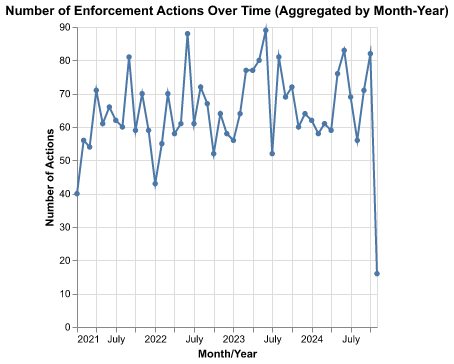
\includegraphics{line_agg.png}

}

\caption{line\_agg}

\end{figure}%

\paragraph{2. (Partner 1) Plot a line chart that shows: the number of
enforcement actions split out by: • ``Criminal and Civil Actions''
vs.~``State Enforcement Agencies'' • Five topics in the ``Criminal and
Civil Actions'' category: ``Health Care Fraud'', ``Financial Fraud'',
``Drug Enforcement'', ``Bribery/Corruption'', and
``Other''.}\label{partner-1-plot-a-line-chart-that-shows-the-number-of-enforcement-actions-split-out-by-criminal-and-civil-actions-vs.-state-enforcement-agencies-five-topics-in-the-criminal-and-civil-actions-category-health-care-fraud-financial-fraud-drug-enforcement-briberycorruption-and-other.}

\begin{Shaded}
\begin{Highlighting}[]
\CommentTok{\#\#\# subset for criminal vs state}
\NormalTok{twenty\_one1 }\OperatorTok{=}\NormalTok{ twenty\_one[twenty\_one[}\StringTok{\textquotesingle{}Category\textquotesingle{}}\NormalTok{].isin([}\StringTok{\textquotesingle{}State Enforcement Agencies\textquotesingle{}}\NormalTok{, }\StringTok{\textquotesingle{}Criminal and Civil Actions\textquotesingle{}}\NormalTok{])]}
\NormalTok{dfQ2\_2\_1 }\OperatorTok{=}\NormalTok{ twenty\_one1.groupby([}\StringTok{\textquotesingle{}Month\_Year\textquotesingle{}}\NormalTok{, }\StringTok{\textquotesingle{}Category\textquotesingle{}}\NormalTok{]).size().reset\_index(name}\OperatorTok{=}\StringTok{\textquotesingle{}Count\textquotesingle{}}\NormalTok{)}

\NormalTok{chartQ2\_2\_1 }\OperatorTok{=}\NormalTok{ alt.Chart(dfQ2\_2\_1).mark\_line(point }\OperatorTok{=} \VariableTok{True}\NormalTok{).encode(}
\NormalTok{  x }\OperatorTok{=}\NormalTok{ alt.X(}\StringTok{\textquotesingle{}Month\_Year:T\textquotesingle{}}\NormalTok{, title }\OperatorTok{=} \StringTok{\textquotesingle{}Month/Year\textquotesingle{}}\NormalTok{),}
\NormalTok{  y }\OperatorTok{=}\NormalTok{ alt.Y(}\StringTok{\textquotesingle{}Count:Q\textquotesingle{}}\NormalTok{, title }\OperatorTok{=} \StringTok{\textquotesingle{}Number of Actions\textquotesingle{}}\NormalTok{),}
\NormalTok{  color}\OperatorTok{=}\StringTok{\textquotesingle{}Category:N\textquotesingle{}}\NormalTok{,}
\NormalTok{  tooltip}\OperatorTok{=}\NormalTok{[}\StringTok{\textquotesingle{}Month\_Year:T\textquotesingle{}}\NormalTok{, }\StringTok{\textquotesingle{}Count:Q\textquotesingle{}}\NormalTok{]}
\NormalTok{).properties( title }\OperatorTok{=} \StringTok{\textquotesingle{}Number of Enforcement Actions By Criminal and Civil, VS State Enforcement\textquotesingle{}}\NormalTok{)}

\NormalTok{chartQ2\_2\_1.save(}\StringTok{"chartQ2\_2\_1.png"}\NormalTok{)}
\end{Highlighting}
\end{Shaded}

\begin{figure}[H]

{\centering 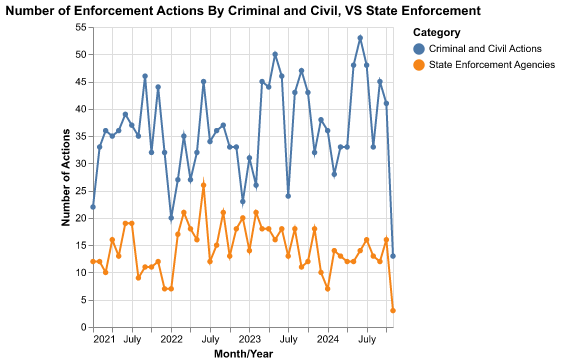
\includegraphics{chartQ2_2_1.png}

}

\caption{chartQ2\_2\_1}

\end{figure}%

\begin{Shaded}
\begin{Highlighting}[]
\CommentTok{\#\#\# subset and categrozie for types of fraud (topics)}
\NormalTok{twenty\_one2 }\OperatorTok{=}\NormalTok{ twenty\_one.copy()}
\NormalTok{twenty\_one2[}\StringTok{\textquotesingle{}Topic\textquotesingle{}}\NormalTok{]}\OperatorTok{=} \VariableTok{None}

\CommentTok{\#\#\# fucntcion filter}
\KeywordTok{def}\NormalTok{ categorize\_topic(text):}
    \ControlFlowTok{if} \StringTok{\textquotesingle{}Health\textquotesingle{}} \KeywordTok{in}\NormalTok{ text }\KeywordTok{or} \StringTok{\textquotesingle{}Medicare\textquotesingle{}} \KeywordTok{in}\NormalTok{ text }\KeywordTok{or} \StringTok{\textquotesingle{}Medicaid\textquotesingle{}} \KeywordTok{in}\NormalTok{ text:}
        \ControlFlowTok{return} \StringTok{\textquotesingle{}Health Care Fraud\textquotesingle{}}
    \ControlFlowTok{elif} \StringTok{\textquotesingle{}Finance\textquotesingle{}} \KeywordTok{in}\NormalTok{ text }\KeywordTok{or} \StringTok{\textquotesingle{}Financial\textquotesingle{}} \KeywordTok{in}\NormalTok{ text }\KeywordTok{or} \StringTok{\textquotesingle{}Monetary\textquotesingle{}} \KeywordTok{in}\NormalTok{ text:}
        \ControlFlowTok{return} \StringTok{\textquotesingle{}Financial Fraud\textquotesingle{}}
    \ControlFlowTok{elif} \StringTok{\textquotesingle{}Drug\textquotesingle{}} \KeywordTok{in}\NormalTok{ text }\KeywordTok{or} \StringTok{\textquotesingle{}Medicine\textquotesingle{}} \KeywordTok{in}\NormalTok{ text }\KeywordTok{or} \StringTok{\textquotesingle{}Prescribe\textquotesingle{}} \KeywordTok{in}\NormalTok{ text }\KeywordTok{or} \StringTok{\textquotesingle{}Prescribing\textquotesingle{}} \KeywordTok{in}\NormalTok{ text:}
        \ControlFlowTok{return} \StringTok{\textquotesingle{}Drug Enforcement\textquotesingle{}}
    \ControlFlowTok{elif} \StringTok{\textquotesingle{}Bribe\textquotesingle{}} \KeywordTok{in}\NormalTok{ text }\KeywordTok{or} \StringTok{\textquotesingle{}Bribery\textquotesingle{}} \KeywordTok{in}\NormalTok{ text }\KeywordTok{or} \StringTok{\textquotesingle{}Corruption\textquotesingle{}} \KeywordTok{in}\NormalTok{ text:}
        \ControlFlowTok{return} \StringTok{\textquotesingle{}Bribery/Corruption\textquotesingle{}}
    \ControlFlowTok{else}\NormalTok{:}
        \ControlFlowTok{return} \StringTok{\textquotesingle{}Other\textquotesingle{}}

\NormalTok{twenty\_one2[}\StringTok{\textquotesingle{}Topic\textquotesingle{}}\NormalTok{] }\OperatorTok{=}\NormalTok{ twenty\_one2[}\StringTok{\textquotesingle{}Title\textquotesingle{}}\NormalTok{].}\BuiltInTok{apply}\NormalTok{(categorize\_topic)}
\end{Highlighting}
\end{Shaded}

\begin{Shaded}
\begin{Highlighting}[]
\CommentTok{\#\#\# plot}
\NormalTok{dfQ2\_2\_2 }\OperatorTok{=}\NormalTok{ twenty\_one2.groupby([}\StringTok{\textquotesingle{}Month\_Year\textquotesingle{}}\NormalTok{, }\StringTok{\textquotesingle{}Topic\textquotesingle{}}\NormalTok{]).size().reset\_index(name}\OperatorTok{=}\StringTok{\textquotesingle{}Count\textquotesingle{}}\NormalTok{)}

\NormalTok{chartQ2\_2\_2 }\OperatorTok{=}\NormalTok{ alt.Chart(dfQ2\_2\_2).mark\_line(point }\OperatorTok{=} \VariableTok{True}\NormalTok{).encode(}
\NormalTok{  x }\OperatorTok{=}\NormalTok{ alt.X(}\StringTok{\textquotesingle{}Month\_Year:T\textquotesingle{}}\NormalTok{, title }\OperatorTok{=} \StringTok{\textquotesingle{}Month/Year\textquotesingle{}}\NormalTok{),}
\NormalTok{  y }\OperatorTok{=}\NormalTok{ alt.Y(}\StringTok{\textquotesingle{}Count:Q\textquotesingle{}}\NormalTok{, title }\OperatorTok{=} \StringTok{\textquotesingle{}Number of Actions\textquotesingle{}}\NormalTok{),}
\NormalTok{  color}\OperatorTok{=}\StringTok{\textquotesingle{}Topic:N\textquotesingle{}}\NormalTok{,}
\NormalTok{  tooltip}\OperatorTok{=}\NormalTok{[}\StringTok{\textquotesingle{}Month\_Year:T\textquotesingle{}}\NormalTok{, }\StringTok{\textquotesingle{}Count:Q\textquotesingle{}}\NormalTok{]}
\NormalTok{).properties( title }\OperatorTok{=} \StringTok{\textquotesingle{}Number of Enforcement Actions By Topic of Fraud\textquotesingle{}}\NormalTok{)}

\NormalTok{chartQ2\_2\_2.save(}\StringTok{"chartQ2\_2\_2.png"}\NormalTok{)}
\end{Highlighting}
\end{Shaded}

\begin{figure}[H]

{\centering 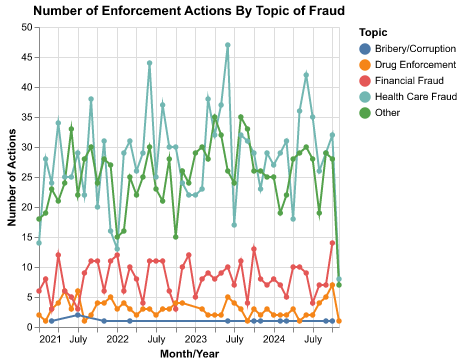
\includegraphics{chartQ2_2_2.png}

}

\caption{chartQ2\_2\_2}

\end{figure}%

\subsection{(15 points) Step 4: Create maps of enforcement activity For
these questions, use this US Attorney District shapefile (link) and a
Census state shapefile
(link)}\label{points-step-4-create-maps-of-enforcement-activity-for-these-questions-use-this-us-attorney-district-shapefile-link-and-a-census-state-shapefile-link}

\paragraph{1. (Partner 1) Map by state: Among actions taken by
state-level agencies, clean the state names you collected and plot a
choropleth of the number of enforcement actions for each state. Hint:
look for ``State of'' in the agency
info!}\label{partner-1-map-by-state-among-actions-taken-by-state-level-agencies-clean-the-state-names-you-collected-and-plot-a-choropleth-of-the-number-of-enforcement-actions-for-each-state.-hint-look-for-state-of-in-the-agency-info}

\begin{Shaded}
\begin{Highlighting}[]
\CommentTok{\#os.chdir(\textquotesingle{}/Users/willsigal/Desktop\textquotesingle{}) \#will wd}
\NormalTok{os.chdir(}\StringTok{\textquotesingle{}d:}\CharTok{\textbackslash{}\textbackslash{}}\StringTok{UChicago}\CharTok{\textbackslash{}\textbackslash{}}\StringTok{Classes}\CharTok{\textbackslash{}\textbackslash{}}\StringTok{2024Qfall}\CharTok{\textbackslash{}\textbackslash{}}\StringTok{Programming Python}\CharTok{\textbackslash{}\textbackslash{}}\StringTok{problem{-}set{-}5}\CharTok{\textbackslash{}\textbackslash{}}\StringTok{Shapefiles\textquotesingle{}}\NormalTok{) }\CommentTok{\#andy wd}

\NormalTok{state }\OperatorTok{=}\NormalTok{ gpd.read\_file(}\StringTok{\textquotesingle{}cb\_2018\_us\_state\_500k/cb\_2018\_us\_state\_500k.shp\textquotesingle{}}\NormalTok{)}
\NormalTok{state\_geometries }\OperatorTok{=}\NormalTok{ state[}\StringTok{\textquotesingle{}geometry\textquotesingle{}}\NormalTok{]}
\end{Highlighting}
\end{Shaded}

\begin{Shaded}
\begin{Highlighting}[]
\CommentTok{\#\#\# df of state gdf}
\NormalTok{state\_df }\OperatorTok{=}\NormalTok{ pd.DataFrame(state)}

\CommentTok{\#\#\# subset scraped df to state agency only}
\NormalTok{twenty\_one\_Q4\_1 }\OperatorTok{=}\NormalTok{ twenty\_one[twenty\_one[}\StringTok{\textquotesingle{}Agency\textquotesingle{}}\NormalTok{].}\BuiltInTok{str}\NormalTok{.contains(}\StringTok{\textquotesingle{}State\textquotesingle{}}\NormalTok{, na}\OperatorTok{=}\VariableTok{False}\NormalTok{)].copy()}

\CommentTok{\#\#\# subset to only agencies with state in their names via state\_df}
\KeywordTok{def}\NormalTok{ find\_state(title):}
    \ControlFlowTok{for}\NormalTok{ state }\KeywordTok{in}\NormalTok{ state\_df[}\StringTok{\textquotesingle{}NAME\textquotesingle{}}\NormalTok{]:}
        \ControlFlowTok{if}\NormalTok{ state }\KeywordTok{in}\NormalTok{ title:}
            \ControlFlowTok{return}\NormalTok{ state}
    \ControlFlowTok{return} \VariableTok{None}

\NormalTok{twenty\_one\_Q4\_1[}\StringTok{\textquotesingle{}State\textquotesingle{}}\NormalTok{] }\OperatorTok{=}\NormalTok{ twenty\_one\_Q4\_1[}\StringTok{\textquotesingle{}Agency\textquotesingle{}}\NormalTok{].}\BuiltInTok{apply}\NormalTok{(find\_state)}

\CommentTok{\#\#\# groupby}
\NormalTok{twenty\_one\_Q4\_1\_grouped }\OperatorTok{=}\NormalTok{ twenty\_one\_Q4\_1.groupby(}\StringTok{\textquotesingle{}State\textquotesingle{}}\NormalTok{).size().reset\_index(name}\OperatorTok{=}\StringTok{\textquotesingle{}Count\textquotesingle{}}\NormalTok{)}
\NormalTok{twenty\_one\_Q4\_1\_grouped }\OperatorTok{=}\NormalTok{ twenty\_one\_Q4\_1\_grouped.rename(columns}\OperatorTok{=}\NormalTok{\{}\StringTok{\textquotesingle{}State\textquotesingle{}}\NormalTok{: }\StringTok{\textquotesingle{}NAME\textquotesingle{}}\NormalTok{\})}

\CommentTok{\#\#\# merge into state gpd}
\NormalTok{state\_merged }\OperatorTok{=}\NormalTok{ state.merge(twenty\_one\_Q4\_1\_grouped, on}\OperatorTok{=}\StringTok{\textquotesingle{}NAME\textquotesingle{}}\NormalTok{, how}\OperatorTok{=}\StringTok{\textquotesingle{}left\textquotesingle{}}\NormalTok{)}
\NormalTok{state\_merged[}\StringTok{\textquotesingle{}Count\textquotesingle{}}\NormalTok{] }\OperatorTok{=}\NormalTok{ state\_merged[}\StringTok{\textquotesingle{}Count\textquotesingle{}}\NormalTok{].fillna(}\DecValTok{0}\NormalTok{)}
\NormalTok{state\_merged\_test }\OperatorTok{=}\NormalTok{ pd.DataFrame(state\_merged)}
\end{Highlighting}
\end{Shaded}

\begin{Shaded}
\begin{Highlighting}[]
\NormalTok{ig, ax }\OperatorTok{=}\NormalTok{ plt.subplots(figsize}\OperatorTok{=}\NormalTok{(}\DecValTok{12}\NormalTok{, }\DecValTok{8}\NormalTok{))  }
\NormalTok{state\_merged.plot(}
\NormalTok{    column}\OperatorTok{=}\StringTok{\textquotesingle{}Count\textquotesingle{}}\NormalTok{, }
\NormalTok{    cmap}\OperatorTok{=}\StringTok{\textquotesingle{}viridis\textquotesingle{}}\NormalTok{, }
\NormalTok{    legend}\OperatorTok{=}\VariableTok{True}\NormalTok{, }
\NormalTok{    ax}\OperatorTok{=}\NormalTok{ax,}
\NormalTok{    edgecolor}\OperatorTok{=}\StringTok{\textquotesingle{}black\textquotesingle{}}\NormalTok{,  }\CommentTok{\# Add borders for clarity}
\NormalTok{    linewidth}\OperatorTok{=}\FloatTok{0.5}\NormalTok{)}
\NormalTok{ax.set\_title(}\StringTok{\textquotesingle{}Enforcement Actions by State\textquotesingle{}}\NormalTok{, fontsize}\OperatorTok{=}\DecValTok{14}\NormalTok{)}
\CommentTok{\#Removed Alska as it made the graph look horrible}
\NormalTok{ax.set\_xlim([}\OperatorTok{{-}}\DecValTok{130}\NormalTok{, }\OperatorTok{{-}}\DecValTok{65}\NormalTok{])}
\NormalTok{ax.set\_ylim([}\DecValTok{24}\NormalTok{, }\DecValTok{50}\NormalTok{])}
\NormalTok{plt.show()}
\end{Highlighting}
\end{Shaded}

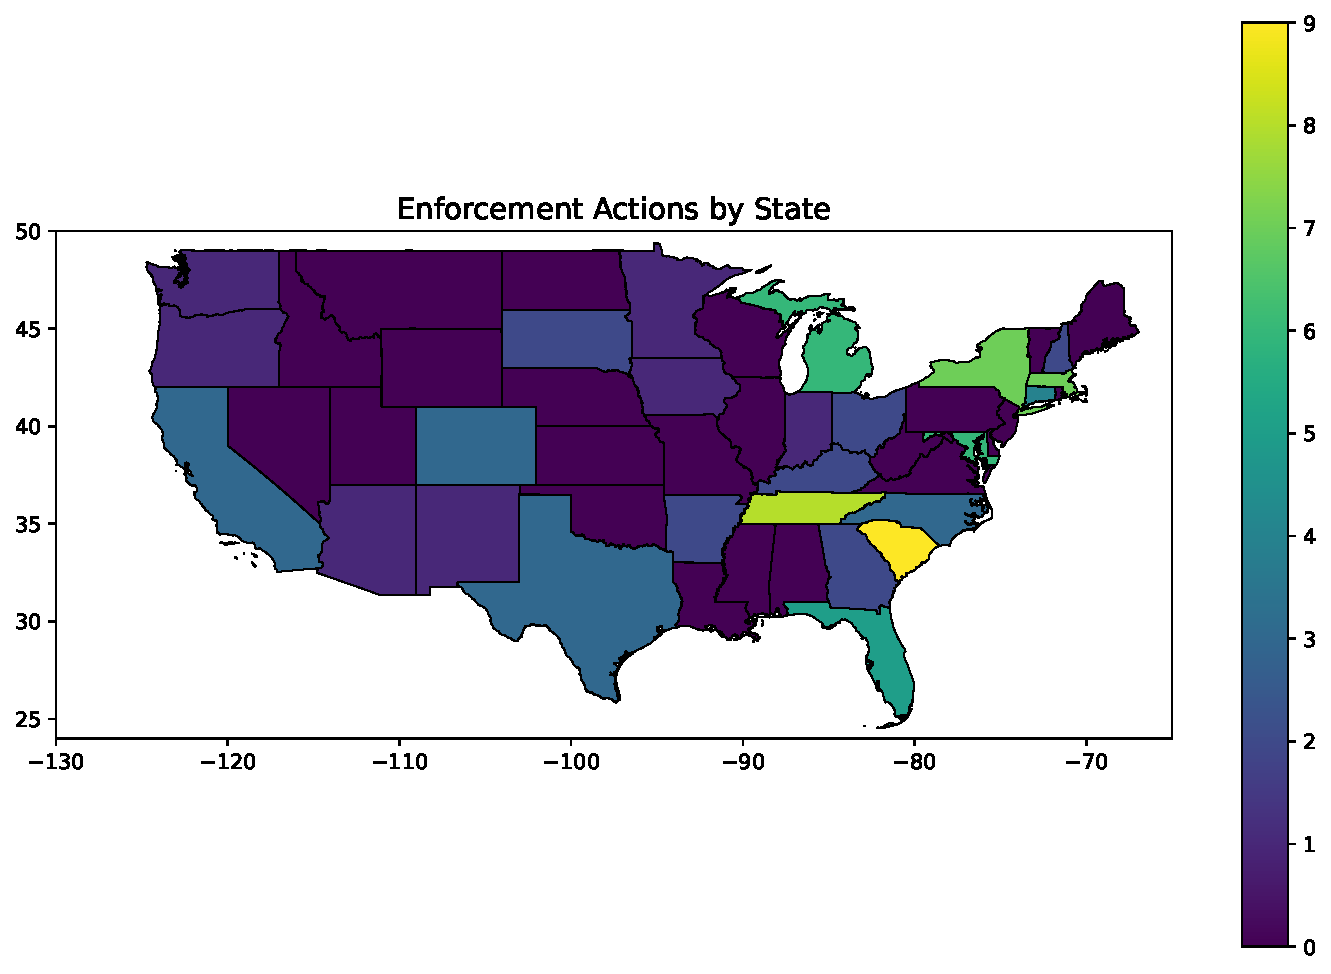
\includegraphics{ps5_files/figure-pdf/cell-23-output-1.pdf}

\paragraph{2. (Partner 2) Map by district: Among actions taken by US
Attorney District-level agencies, clean the district names so that you
can merge them with the shapefile, and then plot a choropleth of the
number of enforcement actions in each US Attorney District. Hint: look
for ``District'' in the agency
info.}\label{partner-2-map-by-district-among-actions-taken-by-us-attorney-district-level-agencies-clean-the-district-names-so-that-you-can-merge-them-with-the-shapefile-and-then-plot-a-choropleth-of-the-number-of-enforcement-actions-in-each-us-attorney-district.-hint-look-for-district-in-the-agency-info.}

\begin{Shaded}
\begin{Highlighting}[]
\CommentTok{\#os.chdir(\textquotesingle{}/Users/willsigal/Desktop/US Attorney Districts Shapefile simplified\_20241108\textquotesingle{}) \#will wd}
\CommentTok{\#districts\_gdf = gpd.read\_file(\textquotesingle{}geo\_export\_6b570657{-}b5c6{-}4bbc{-}b83a{-}415e4880d085.shp\textquotesingle{}) \#will import}

\NormalTok{os.chdir(}\StringTok{\textquotesingle{}d:}\CharTok{\textbackslash{}\textbackslash{}}\StringTok{UChicago}\CharTok{\textbackslash{}\textbackslash{}}\StringTok{Classes}\CharTok{\textbackslash{}\textbackslash{}}\StringTok{2024Qfall}\CharTok{\textbackslash{}\textbackslash{}}\StringTok{Programming Python}\CharTok{\textbackslash{}\textbackslash{}}\StringTok{problem{-}set{-}5}\CharTok{\textbackslash{}\textbackslash{}}\StringTok{Shapefiles}\CharTok{\textbackslash{}\textbackslash{}}\StringTok{US Attorney Districts Shapefile simplified\_20241109\textquotesingle{}}\NormalTok{) }\CommentTok{\#andy wd}
\NormalTok{districts\_gdf }\OperatorTok{=}\NormalTok{ gpd.read\_file(}\StringTok{\textquotesingle{}geo\_export\_5d56b225{-}6390{-}4cf1{-}bb2b{-}122a8672faf1.shp\textquotesingle{}}\NormalTok{) }\CommentTok{\#andy import}

\NormalTok{district\_df }\OperatorTok{=}\NormalTok{ pd.DataFrame(districts\_gdf)}
\end{Highlighting}
\end{Shaded}

\begin{Shaded}
\begin{Highlighting}[]
\NormalTok{district\_twentyone\_df }\OperatorTok{=}\NormalTok{ twenty\_one[twenty\_one[}\StringTok{\textquotesingle{}Agency\textquotesingle{}}\NormalTok{].}\BuiltInTok{str}\NormalTok{.contains(}\StringTok{\textquotesingle{}District\textquotesingle{}}\NormalTok{, na}\OperatorTok{=}\VariableTok{False}\NormalTok{)].copy()}
\end{Highlighting}
\end{Shaded}

\begin{Shaded}
\begin{Highlighting}[]
\NormalTok{district\_df.head}
\end{Highlighting}
\end{Shaded}

\begin{verbatim}
<bound method NDFrame.head of    statefp                             judicial_d         aland        awater  \
0       21           Western District of Kentucky  4.970555e+10  1.651516e+09   
1       21           Eastern District of Kentucky  5.257394e+10  7.238213e+08   
2       18           Southern District of Indiana  5.824517e+10  5.941176e+08   
3       01             Middle District of Alabama  3.412673e+10  5.472423e+08   
4       01           Southern District of Alabama  6.235882e+10  3.052681e+09   
..     ...                                    ...           ...           ...   
89      69  District of Northern Marianas Islands  4.722925e+08  4.644252e+09   
90      12           Southern District of Florida  2.448809e+10  1.159277e+10   
91      40          Northern District of Oklahoma  2.231989e+10  7.189768e+08   
92      50                    District of Vermont  2.387418e+10  1.030417e+09   
93      10                   District of Delaware  5.045926e+09  1.399986e+09   

                        state           chief_judg            nominating  \
0                    Kentucky      Greg N. Stivers      Barack Obama (D)   
1                    Kentucky         Danny Reeves    George W. Bush (R)   
2                     Indiana  Jane Magnus-Stinson      Barack Obama (D)   
3                     Alabama    Emily Coody Marks      Donald Trump (R)   
4                     Alabama        Kristi DuBose    George W. Bush (R)   
..                        ...                  ...                   ...   
89  Northern Marianas Islands   Ramona V. Manglona      Barack Obama (D)   
90                    Florida     K. Michael Moore  George H.W. Bush (R)   
91                   Oklahoma         John Dowdell      Barack Obama (D)   
92                    Vermont    Geoffrey Crawford      Barack Obama (D)   
93                   Delaware        Leonard Stark      Barack Obama (D)   

    term_as_ch  shape_leng  shape_area abbr district_n    shape__are  \
0       2018.0   16.200585    5.216899  KYW          6  8.123902e+10   
1       2019.0   13.514251    5.451047  KYE          6  8.547129e+10   
2       2016.0   14.956126    6.137433  INS          7  9.818187e+10   
3       2019.0   10.235799    3.858442  ALM         11  5.645450e+10   
4       2017.0   12.976906    3.278871  ALS         11  4.772733e+10   
..         ...         ...         ...  ...        ...           ...   
89      2011.0    3.252892    0.040335   MP          9  5.200276e+08   
90      2014.0   17.941594    2.503158  FLS         11  3.466156e+10   
91      2019.0    8.154257    2.316496  OKN         10  3.569729e+10   
92      2017.0    9.571257    2.797955   VT          2  4.826994e+10   
93      2014.0    4.285079    0.541590   DE          3  8.634830e+09   

      shape__len                                           geometry  
0   1.964255e+06  MULTIPOLYGON (((-89.48248 36.50214, -89.48543 ...  
1   1.654681e+06  POLYGON ((-84.62012 39.07346, -84.60793 39.073...  
2   1.887626e+06  POLYGON ((-85.86281 40.46476, -85.86212 40.406...  
3   1.236201e+06  POLYGON ((-85.33828 33.49471, -85.33396 33.492...  
4   1.567095e+06  MULTIPOLYGON (((-88.08682 30.25987, -88.07676 ...  
..           ...                                                ...  
89  3.702108e+05  MULTIPOLYGON (((145.28433 14.17537, 145.28404 ...  
90  2.117424e+06  MULTIPOLYGON (((-81.9667 24.52376, -81.97837 2...  
91  9.857548e+05  POLYGON ((-95.04951 36.99959, -95.03786 36.999...  
92  1.248962e+06  POLYGON ((-72.67477 45.01547, -72.58988 45.013...  
93  5.622177e+05  MULTIPOLYGON (((-75.56246 39.51266, -75.56745 ...  

[94 rows x 15 columns]>
\end{verbatim}

\begin{Shaded}
\begin{Highlighting}[]
\CommentTok{\#removing the prefixes}
\NormalTok{district\_twentyone\_df[}\StringTok{\textquotesingle{}District\textquotesingle{}}\NormalTok{] }\OperatorTok{=}\NormalTok{ district\_twentyone\_df[}\StringTok{\textquotesingle{}Agency\textquotesingle{}}\NormalTok{].}\BuiltInTok{apply}\NormalTok{(}\KeywordTok{lambda}\NormalTok{ x: x.split(}\StringTok{\textquotesingle{}, \textquotesingle{}}\NormalTok{)[}\OperatorTok{{-}}\DecValTok{1}\NormalTok{] }\ControlFlowTok{if} \StringTok{\textquotesingle{}, \textquotesingle{}} \KeywordTok{in}\NormalTok{ x }\ControlFlowTok{else}\NormalTok{ x)}
\NormalTok{district\_twentyone\_df[}\StringTok{\textquotesingle{}District\textquotesingle{}}\NormalTok{] }\OperatorTok{=}\NormalTok{ district\_twentyone\_df[}\StringTok{\textquotesingle{}District\textquotesingle{}}\NormalTok{].}\BuiltInTok{str}\NormalTok{.strip()}

\NormalTok{district\_twentyone\_df[}\StringTok{\textquotesingle{}District\textquotesingle{}}\NormalTok{] }\OperatorTok{=}\NormalTok{ district\_twentyone\_df[}\StringTok{\textquotesingle{}District\textquotesingle{}}\NormalTok{].}\BuiltInTok{str}\NormalTok{.replace(}\StringTok{\textquotesingle{}U.S. Attorney}\CharTok{\textbackslash{}\textquotesingle{}}\StringTok{s Office, \textquotesingle{}}\NormalTok{, }\StringTok{\textquotesingle{}\textquotesingle{}}\NormalTok{)}

\NormalTok{district\_twentyone\_df[}\StringTok{\textquotesingle{}District\textquotesingle{}}\NormalTok{].head}
\end{Highlighting}
\end{Shaded}

\begin{verbatim}
<bound method NDFrame.head of 1                  District of Idaho
2          District of Massachusetts
3       Eastern District of Virginia
4         Middle District of Florida
5          Western District of Texas
                    ...             
3016             District of Montana
3017              District of Alaska
3018          District of New Jersey
3020          District of New Jersey
3021    Middle District of Tennessee
Name: District, Length: 1413, dtype: object>
\end{verbatim}

\begin{Shaded}
\begin{Highlighting}[]
\NormalTok{enforcement\_counts }\OperatorTok{=}\NormalTok{ district\_twentyone\_df[}\StringTok{\textquotesingle{}District\textquotesingle{}}\NormalTok{].value\_counts().reset\_index()}
\NormalTok{enforcement\_counts.columns }\OperatorTok{=}\NormalTok{ [}\StringTok{\textquotesingle{}District\textquotesingle{}}\NormalTok{, }\StringTok{\textquotesingle{}Enforcement Actions\textquotesingle{}}\NormalTok{]}
\end{Highlighting}
\end{Shaded}

\begin{Shaded}
\begin{Highlighting}[]
\NormalTok{merged\_districts\_df }\OperatorTok{=}\NormalTok{ pd.merge(district\_df, enforcement\_counts, left\_on}\OperatorTok{=}\StringTok{\textquotesingle{}judicial\_d\textquotesingle{}}\NormalTok{, right\_on}\OperatorTok{=}\StringTok{\textquotesingle{}District\textquotesingle{}}\NormalTok{, how}\OperatorTok{=}\StringTok{\textquotesingle{}left\textquotesingle{}}\NormalTok{)}

\NormalTok{merged\_districts\_df[}\StringTok{\textquotesingle{}Enforcement Actions\textquotesingle{}}\NormalTok{] }\OperatorTok{=}\NormalTok{ merged\_districts\_df[}\StringTok{\textquotesingle{}Enforcement Actions\textquotesingle{}}\NormalTok{].fillna(}\DecValTok{0}\NormalTok{)}
\NormalTok{merged\_districts\_df.columns}
\end{Highlighting}
\end{Shaded}

\begin{verbatim}
Index(['statefp', 'judicial_d', 'aland', 'awater', 'state', 'chief_judg',
       'nominating', 'term_as_ch', 'shape_leng', 'shape_area', 'abbr',
       'district_n', 'shape__are', 'shape__len', 'geometry', 'District',
       'Enforcement Actions'],
      dtype='object')
\end{verbatim}

\begin{Shaded}
\begin{Highlighting}[]
\NormalTok{gdf }\OperatorTok{=}\NormalTok{ gpd.GeoDataFrame(merged\_districts\_df, geometry}\OperatorTok{=}\StringTok{\textquotesingle{}geometry\textquotesingle{}}\NormalTok{)}
\BuiltInTok{print}\NormalTok{(gdf.crs)}
\NormalTok{gdf[}\StringTok{\textquotesingle{}Enforcement Actions\textquotesingle{}}\NormalTok{] }\OperatorTok{=}\NormalTok{ gdf[}\StringTok{\textquotesingle{}Enforcement Actions\textquotesingle{}}\NormalTok{].fillna(}\DecValTok{0}\NormalTok{)}
\end{Highlighting}
\end{Shaded}

\begin{verbatim}
EPSG:4326
\end{verbatim}

\begin{Shaded}
\begin{Highlighting}[]
\NormalTok{ig, ax }\OperatorTok{=}\NormalTok{ plt.subplots(figsize}\OperatorTok{=}\NormalTok{(}\DecValTok{12}\NormalTok{, }\DecValTok{8}\NormalTok{))  }\CommentTok{\# Adjust figure size}
\NormalTok{gdf.plot(}
\NormalTok{    column}\OperatorTok{=}\StringTok{\textquotesingle{}Enforcement Actions\textquotesingle{}}\NormalTok{, }
\NormalTok{    cmap}\OperatorTok{=}\StringTok{\textquotesingle{}viridis\textquotesingle{}}\NormalTok{, }
\NormalTok{    legend}\OperatorTok{=}\VariableTok{True}\NormalTok{, }
\NormalTok{    ax}\OperatorTok{=}\NormalTok{ax,}
\NormalTok{    edgecolor}\OperatorTok{=}\StringTok{\textquotesingle{}black\textquotesingle{}}\NormalTok{,  }\CommentTok{\# Add borders for clarity}
\NormalTok{    linewidth}\OperatorTok{=}\FloatTok{0.5}\NormalTok{)}
\NormalTok{ax.set\_title(}\StringTok{\textquotesingle{}Enforcement Actions by Judicial District\textquotesingle{}}\NormalTok{, fontsize}\OperatorTok{=}\DecValTok{14}\NormalTok{)}
\CommentTok{\#Removed Alska as it made the graph look horrible}
\NormalTok{ax.set\_xlim([}\OperatorTok{{-}}\DecValTok{130}\NormalTok{, }\OperatorTok{{-}}\DecValTok{65}\NormalTok{])}
\NormalTok{ax.set\_ylim([}\DecValTok{24}\NormalTok{, }\DecValTok{50}\NormalTok{])}
\NormalTok{plt.show()}
\end{Highlighting}
\end{Shaded}

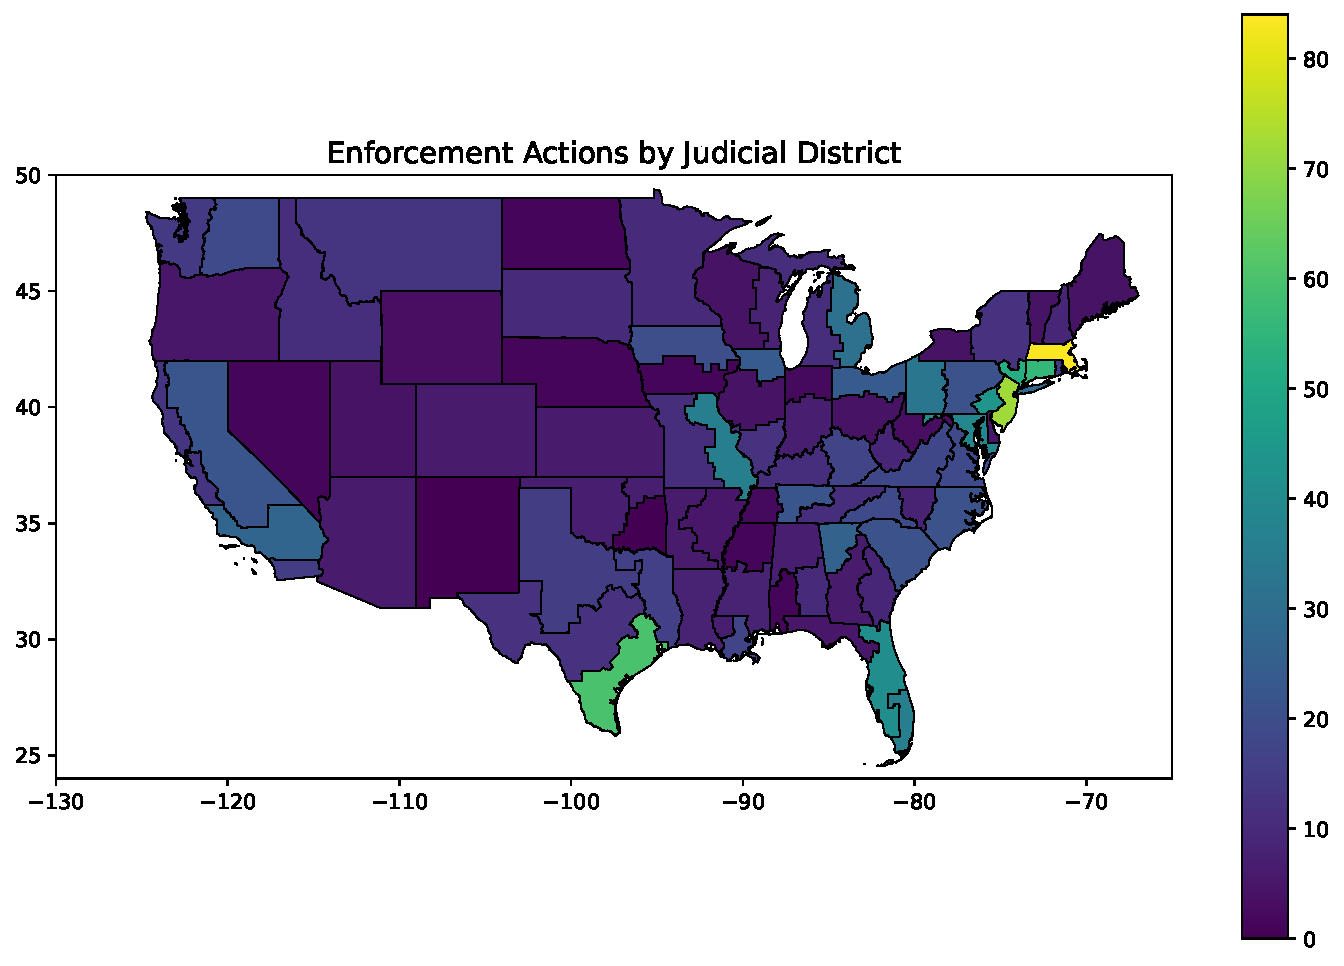
\includegraphics{ps5_files/figure-pdf/cell-31-output-1.pdf}

\subsection{(10 points) Extra credit: Calculate the enforcement actions
on a per-capita basis (Both partners can work
together)}\label{points-extra-credit-calculate-the-enforcement-actions-on-a-per-capita-basis-both-partners-can-work-together}

\paragraph{1. Use the zip code shapefile from the previous problem set
and merge it with zip code level population data. (Go to Census Data
Portal, select ``ZIP Code Tabulation Area'', check ``All 5-digit ZIP
Code Tabulation Areas within United States'', and under ``P1 TOTAL
POPULATION'' select ``2020: DEC Demographic and Housing
Characteristics''. Download the
csv.).}\label{use-the-zip-code-shapefile-from-the-previous-problem-set-and-merge-it-with-zip-code-level-population-data.-go-to-census-data-portal-select-zip-code-tabulation-area-check-all-5-digit-zip-code-tabulation-areas-within-united-states-and-under-p1-total-population-select-2020-dec-demographic-and-housing-characteristics.-download-the-csv..}

\paragraph{2. Conduct a spatial join between zip code shapefile and the
district shapefile, then aggregate to get population in each
district.}\label{conduct-a-spatial-join-between-zip-code-shapefile-and-the-district-shapefile-then-aggregate-to-get-population-in-each-district.}

\paragraph{3. Mapthe ratio of enforcement actions in each US Attorney
District. You can calculate the ratio by aggregating the number of
enforcement actions since January 2021 per district, and dividing it
with the population
data.}\label{mapthe-ratio-of-enforcement-actions-in-each-us-attorney-district.-you-can-calculate-the-ratio-by-aggregating-the-number-of-enforcement-actions-since-january-2021-per-district-and-dividing-it-with-the-population-data.}




\end{document}
